\documentclass[a4paper,11pt,eval]{nsi} % COMPILE WITH DRAFT
\usepackage{hyperref}

\pagestyle{empty}
\begin{document}

\textcolor{UGLiBlue}{Vendredi 07/03/2025}\\
\classe{\terminale Comp}
\titre{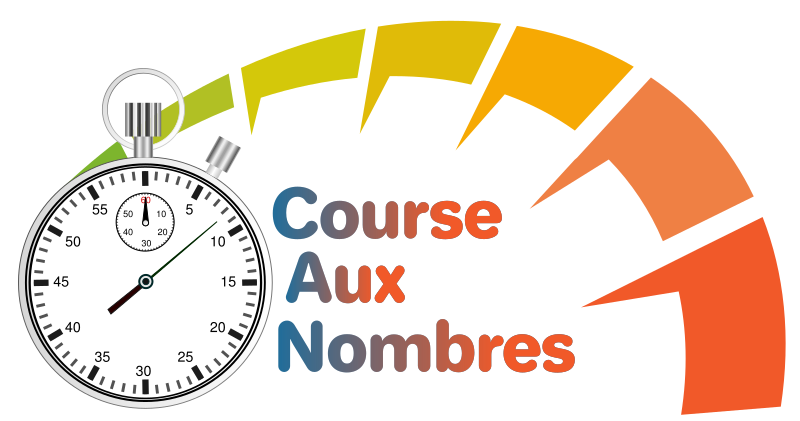
\includegraphics[width=3cm]{CAN.png} Interro 1}
\maketitle



\begin{enumerate}[itemsep=1em]
	\item $4 \times 0{,}7=$  $\ldots$
	\item $4+\dfrac{4}{3}= $ $\ldots$
	\item Développer et réduire l'expression $(3x+4)(5x-2)$.
	\item Donner l'écriture décimale de :  $9\times10^3+4+4\times 10^{-1}$.
	\item Résoudre l'équation $6x+4=0$.
	\item $8$ croissants coûtent  $8{,}80$ €.  Combien coûtent $4$ croissants ?
                        
	\item Calculer la fréquence de boules noires parmi ces boules :\\
          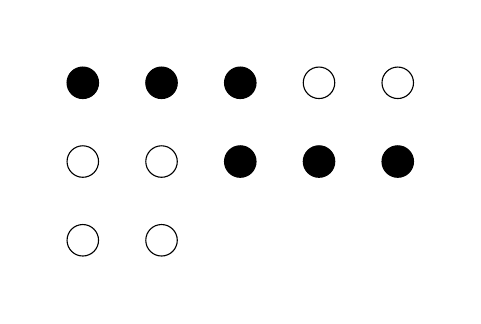
\begin{tikzpicture}[baseline]

    \tikzset{
      point/.style={
        thick,
        draw,
        cross out,
        inner sep=0pt,
        minimum width=5pt,
        minimum height=5pt,
      },
    }
    \clip (-0.7,-2.7) rectangle (4.7,0.7);
    	
	 \filldraw[color={black},fill={black}] (0,0) circle (0.2);
	
	 \filldraw[color={black},fill={black}] (1,0) circle (0.2);
	
	 \filldraw[color={black},fill={black}] (2,0) circle (0.2);
	
	 \filldraw[color={black},fill={white}] (3,0) circle (0.2);
	
	 \filldraw[color={black},fill={white}] (4,0) circle (0.2);
	
	 \filldraw[color={black},fill={white}] (0,-1) circle (0.2);
	
	 \filldraw[color={black},fill={white}] (1,-1) circle (0.2);
	
	 \filldraw[color={black},fill={black}] (2,-1) circle (0.2);
	
	 \filldraw[color={black},fill={black}] (3,-1) circle (0.2);
	
	 \filldraw[color={black},fill={black}] (4,-1) circle (0.2);
	
	 \filldraw[color={black},fill={white}] (0,-2) circle (0.2);
	
	 \filldraw[color={black},fill={white}] (1,-2) circle (0.2);

\end{tikzpicture}\\
	\item Calculer l'expression  $x^2+2x+8$ pour $x=-2$.
	\item Calculer la moyenne de :
            $28\,\,\,; \,\,\,8\,\,\,; \,\,\,32\,\,\,; \,\,\,52$.
	\item $70$ $\%$ de $20= $ $\ldots$
	%\item  $8{,}5$ L $=$ $\ldots$ m$^3$
\end{enumerate}



\vspace*{1cm}
%Mon temps : $\ldots$\\[.5em]
%Mon score : $\ldots$/10

\newpage
\titre{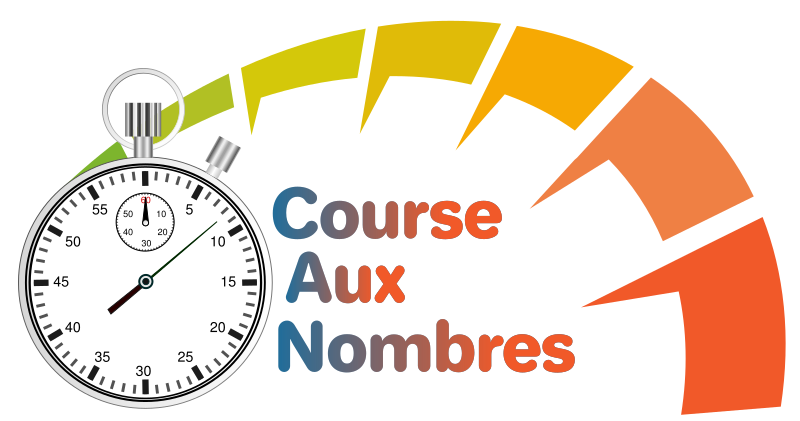
\includegraphics[width=3cm]{CAN.png} Corrigé de l'interro 1}
\maketitle

\textcolor{UGLiBlue}{
    \begin{enumerate}[itemsep=1em]
        \item $4 \times 0{,}7=4\times 7\times 0,1=2{,}8$
        \item $4+\dfrac{4}{3}= \dfrac{12}{3}+\dfrac{4}{3}=\dfrac{16}{3}$
        \item \begin{tabbing}
            $(3x+4)(5x-2)$\=$=3x\times 5x+4\times 5x-2\times 3x-2\times 4$\\
            \>$=15x^2+20x-6x-8$\\
            \>$=15x^2+14x-8$
        \end{tabbing}
        \item $9\times10^3+4+4\times 10^{-1}=9\,000+4+0{,}4=9\,004{,}4$
        \item On se ramène à une équation du type $a\times x=b$ :\\
                  $\begin{aligned}
                  6x+4&=0\\
                 6x&=-4\\
                                      x&=\dfrac{-4}{6}=-\dfrac{2{\color[HTML]{2563a5}\boldsymbol{\times2}} }{3{\color[HTML]{2563a5}\boldsymbol{\times2}}}=-\dfrac{2}{3}
                 \end{aligned}$\\
                  L'équation $6x+4=0$ a pour solution $x=-\dfrac{2}{3}$.
        \item $8$ croissants coûtent  $8{,}80$ €, donc
                               $4$ croissants coûtent $2$ fois moins, soit : \\
                               $8{,}80\div 2=4{,}40$ €.
        \item La fréquence est donnée par le quotient : $\dfrac{\text{Nombre de boules noires}}{\text{Nombre total de boules}}=\dfrac{6}{12}=\dfrac{1{\color[HTML]{2563a5}\boldsymbol{\times6}} }{2{\color[HTML]{2563a5}\boldsymbol{\times6}}}=\dfrac{1}{2}$.
        \item 
                    Pour $x=-2$, on obtient : $x^2+2x+8=(-2)^2+2\times (-2)+8=8$.        
        \item La moyenne est donnée par : $\dfrac{28+8+32+52}{4}=\dfrac{120}{4}=30$.
        \item           Prendre $70$ $\%$  de $20$ revient à prendre $7\times 10$ $\%$  de $20$.\\
                    Comme $10$ $\%$  de $20$ vaut $2$ (pour prendre $10$ $\%$  d'une quantité, on la divise par $10$), alors
                    $70$ $\%$ de $20=7\times 2=14$.
        %\item Comme $1$ L= $0,001$ m$^3$, $8{,}5$ L $=0{,}008\,5$  m$^3$.
\end{enumerate}
}
\end{document}